% !TeX root = ../main.tex

\section{Discret Fourier Transform (DFT)}
Discrete time sequence \textbf{periodic}. Discrete both in time and frequency, finite number/summation:
\begin{LARGE}
    $$
    X(k)=\sum_{n=0}^{N-1} x(n)e^{-j2\pi \frac{k}{N}n}
    $$
\end{LARGE}
$X(k)$ with $k=[0,N-1]$. While DTFT is continuous in the frequency domain
$$
X(f)=\sum_{n=-\infty}^\infty x(n)e^{-j2\pi fn}
$$
\textbf{In the DFT we assume that the period is signal w.r.t. provided N}

\subsection{Relationship with DTFT}
\begin{itemize}
    \item While in DTFT $f\in\,\,[0,1)$, with DFT $f=\left[0,\frac{1}{N},\cdots,\frac{N-1}{N}\right]\rightarrow$ length of $N$
    \item The inverse (IDFT):
    $$
    x(n)=\frac{1}{N}\sum_{k=0}^{N-1}X(k)e^{2j\pi\frac{k}{N}n}
    $$
    Length of $N$
    \item \textbf{DFT==DTFT only if FIR}, if IIR we are truncating when applying DFT, losing info
    \item DTFT continuous over frequencies, DFT discrete
    \begin{itemize}
        \item Sampling in Fourier = periodicity in time
        \item Sampling in time = periodicity in frequency/Fourier
    \end{itemize}
    \item Both DFT and IDFT are periodic with a period of $N$ samples:
    $$
    X(k+tN)=X(k)\qquad\forall\,\,t\in[-\infty,\infty]
    $$
    $$
    x(n)=IDFT(X(k))=x(n+tN)\qquad\forall\,\,t\in[-\infty,\infty]
    $$
\end{itemize}

\subsection{DFT as a matrix product}
The DFT of a sequence $x(n)$ can be computed by:
$$X=W_N\cdot x$$
Where:
$$
W_N=
\begin{bmatrix}
    W_i^0 & W_i^0 & W_i^0 & W_i^0 & \cdots & W_i^0\\
    W_i^0 & W_i^1 & W_i^2 & W_i^3 & \cdots & W_i^{N-1}\\
    W_i^0 & W_i^2 & W_i^4 & W_i^6 & \cdots & W_i^{2(N-1)}\\
    W_i^0 & W_i^3 & W_i^6 & W_i^9 & \cdots & W_i^{3(N-1)}\\
    \vdots & \vdots & \vdots & \vdots & \ddots & \vdots\\
    W_i^0 & W_i^{N-1} & W_i^{2(N-1)} & W_i^{3(N-1)} & \cdots & W_i^{(N-1)^2}        
\end{bmatrix}=
$$
$$
=
\begin{bmatrix}
    1 & 1 & 1 & 1 & 1\\
    1 & e^{-j2\pi/N} & e^{-j4\pi/N} & \cdots & e^{-j2\pi(N-1)/N}\\
    1 & e^{-j4\pi/N} & e^{-j8\pi/N} & \cdots & e^{-j4\pi(N-1)/N}\\
    1 & \cdots & \cdots & \cdots & \cdots\\
    1 & e^{-j2\pi(N-1)/N} & e^{-j4\pi(N-1)/N} & \cdots & e^{-j2\pi(N-1)(N-1)/N}
\end{bmatrix}
$$
\begin{LARGE}
    $$W_i=e^{-j\frac{2\pi}{i}}$$
\end{LARGE}
Or
$$
W_N=e^{-j\frac{2\pi}{N}kn}
$$
$$
\underline{k}=\left[0,1,\cdots,N-1\right]
$$
$$
\underline{n}=\left[0,1,\cdots,N-1\right]
$$
\textbf{The inverse of $W:\,\,N\times N$ is its conjugate transpose divided by $N$}.
$$y(n)=W^{-1}Y(k)$$

\textbf{If using matrices, $Y(k)=X(k)\cdot H(k)$ element-wise product}.

\subsection{Zero padding}
Zero padding means windowing, which will result in a sinc behavior in the Fourier domain. When we compute the DFT, if the repetition of the signal results in discountinuities:
\begin{center}
    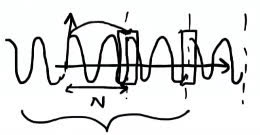
\includegraphics[width=0.5\textwidth]{images/zero_pad_01.png}
\end{center}
We introduce zero till we get a signal that repeated will not have discountinuities. This new signal obtained is made of the product of two signals: itself and a rectangle that ends where the previous signal ended (will become 0 onward, so $N_{pad}$ must be multiple of period)
\begin{center}
    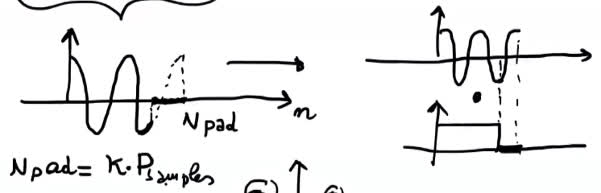
\includegraphics[width=0.8\textwidth]{images/zero_pad_02.png}
\end{center}
In the Fourier/frequency domain so we will get the \textbf{convolution} of transform of those two signals: the transform of the first will be two pulses ($\delta$) at the peaks, while the transform of the rectangle will be a sinc.\\
Convolving the two, we will get two sincs due to the effect of the window, each one the peaks (in the example peaks at $2Hz$ as frequency of sinusoid $f_0=2Hz$):
\begin{center}
    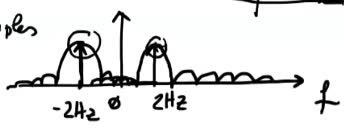
\includegraphics[width=0.5\textwidth]{images/zero_pad_03.png}
\end{center}
But when discretize the DFT, we should be careful to put the peak $x$ in the axis/in the interval plotted:
$$k\frac{F_s}{N_{pad}}=f_0$$
$$N_{pad}=k\frac{F_s}{f_0}=k\cdot P_{samples}$$
Same conclusion as before.

But if \textbf{strong density} in the spectrum (a lot of padded zeros), introducing a sinc and the peak will not be exactly at $f_0$, small overlap on the maximum
due to tails, introduced errors.

\subsubsection{Conditions}
\begin{enumerate}
    \item $N_{pad}=k\cdot P_{samples}$. \textbf{If 2+ signals summed, the global period in samples is the least common multiple (mcm) of the periods}. What if one of the periods is not an integer?
    $$
    \begin{cases}
        P_1=25\\
        P_2=\frac{50}{2.2}=\frac{250}{11}
    \end{cases}
    $$
    $$
    lcm(25,\frac{250}{11})=lcm(25,250)=250
    $$
\end{enumerate}

\subsubsection{Alternative to zero-padding for discountinuities in DFT}
When we are windowing we have a rectangular behavior. If its length is $N$, its first zero is $\frac{1}{N}$
\begin{center}
    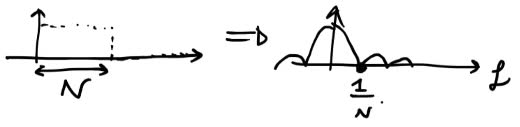
\includegraphics[width=0.7\textwidth]{images/zero_pad_04.png}
\end{center}
Suppose a signal with 50 samples, the size of the main lobe we are introducing in the frequency (the first zero) is $\frac{1}{50}$ in the normalized domain or $\frac{1}{50}F_s$ in the $Hz$ domain. Suppose $F_s=50$:
\begin{center}
    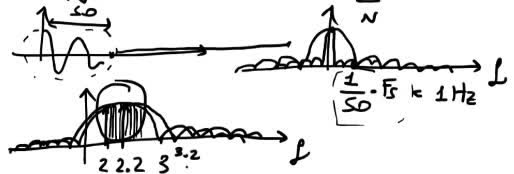
\includegraphics[width=0.7\textwidth]{images/zero_pad_05.png}
\end{center}
Two lobes sum up, so using zero-padding useless. We have to reduce size of main lobe of the sinc: increasing number of samples.
\begin{center}
    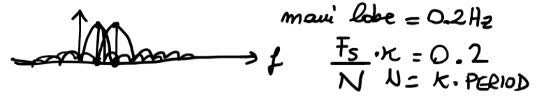
\includegraphics[width=0.7\textwidth]{images/zero_pad_06.png}
\end{center}
So the Alternative is to redefine the signals in time domain with samples equal to the global period in samples immediately: \textbf{more measurement, add more samples}.

\subsection{Discontinuity}
In the Fourier domain introduces high frequency content

\subsection{DFT of sinusoids: pulses and peaks}
A sinusoid (a cosine) with frequency $f_0$ will have two $\delta$'s in the frequency domain, one at $f_0$ the other at $-f_0=F_s-f_0$ (mirrored w.r.t. $F_s/2$ Nyquist, if normalized frequencies, it is at $1-\tilde{f}_0$, $\pm\tilde{\omega}_0$). If we add a second signal with a different frequency $f_0'$, we will have two additions $\delta$'s at $f_0'$ and $-f_0'$. In the magnitude/amplitude plot, the two pulses will have $\frac{N}{2}$ height

Given a sinusoid with $F_s$ [Hz] and $f_0$ [Hz], its DFT will have two peaks, one in $f_0$, the other one in $F_s-f_0$, symmetric w.r.t. the Nyquist frequency. For example, given:
$$
x(t) = A*\cos(2\pi f_0t)\qquad F_s = 50Hz\qquad f_0 = 2Hz
$$
$$
x(n) = A*\cos\left(\frac{2\pi}{25}n\right)
$$
Its DFT is:
$$
|X(\omega)|=\frac{N}{2}\delta\left(\omega-\frac{2\pi}{25}\right)+
\frac{N}{2}\delta\left(\omega-\left(2\pi-\frac{2\pi}{25}\right)\right)
$$

\subsection{DFT and IDFT periodicty}
Given a non periodic sequence $x(n)$ defined over $N$ samples, its $N$-periodic extension is defined as:
$$
\tilde{x}(n)=\sum_{t=-\infty}^\infty x(n-tN)
$$
Same with DFT:
$$
\tilde{X}(k)=\sum_{t=-\infty}^\infty X(k-tN)
$$

\subsubsection{Cyclic/circular convolution}
For the DFT:
$$
X_1(k)\cdot X_2(k) \neq x_1(n)* x_2(n)
$$
$$
IDFT\Brackets{X_1(k)\cdot X_2(k)}= x_1(n)\circledast x_2(n)=\sum_{m=0}^{N-1}x(m)\tilde{y}(n-m)
$$
The cyclic/circular convolution holds
\begin{center}
    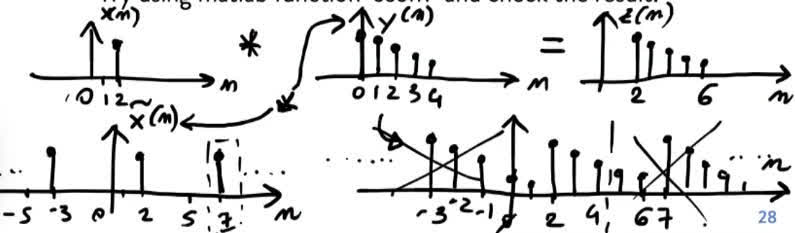
\includegraphics[width=1\textwidth]{images/cyclic_conv.png}
\end{center}
\textbf{So to compute circular convolution I can use the DFT: compute product of DFTs and then invert}.

\textbf{But LTI systems such as communication, radar, audio and image systems all work with linear convolution, so to compute linear convolution in DFT how do we do?}

\subsubsection{Linear and cyclic convolution}
Given a sequence with length $L$ and a sequence with length $P$, the maximum length of the linear convolution is $N_c=L+P-1$.
\begin{center}
    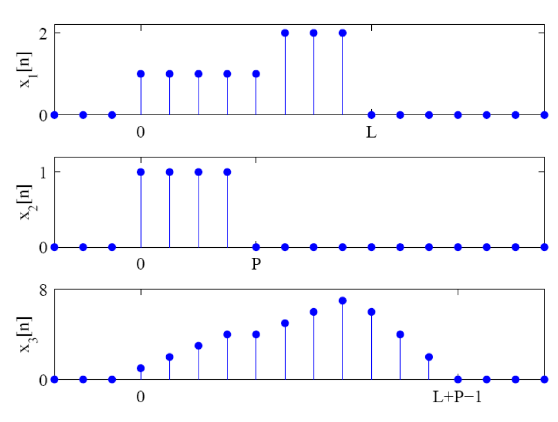
\includegraphics[width=1\textwidth]{images/cyclic_conv_01.png}
\end{center}
The cyclic convolution computed over a generic number $N$ of samples is equal to the linear convolution if $N$ is long enough to avoid periodic artifacts. Therefore
$$
N\geq L+P-1
$$
\textbf{Pad with zeros the two sequences until reaching $N$ samples, we will not introduce artifacts and the result of the cyclic convolution will be equal to that of the normal convolution}.

\subsection{Long convolution}
The input sequence $x(n)$ can be very long, zero-padding can be unfeasible if it is unknown as well (real-time applications), so we can segment the signal into smaller blocks and process them separately

\subsubsection{Overlap and add}
\begin{itemize}
    \item Let the impulse resposne $h(n)$ long $P$, decompose the input $x(n)$ into \textbf{non-overlapped} blocks with length $L$
    \item For each block compute the output as
    $$IDFT(X_n(k)\cdot H(k)),k\in [0,N=L+P-1)$$
    \item Sum the overlapping portions between the results
\end{itemize}

\subsubsection{Overlap and save}
\begin{itemize}
    \item Let the impulse resposne $h(n)$ long $P$, decompose the input $x(n)$ into \textbf{overlapped} blocks with length $L>P$ with overlap $P-1$
    \item The circular convolution evaluated over $L$ sampels is different from the linear convolution only in the first $P-1$ samples (periodic artifacts)
    \item Pad the first block with $P-1$ zeros at the beginning
    \item Overlap blocks by $P-1$ samples
    \item For each block compute the circualr convolution ofer $L$ samples and discard the first $P-1$ samples
    $$IDFT(X_n(k)\cdot H(k)),k\in [0,N=L+P-1)$$
    \item Sum the overlapping portions between the results
\end{itemize}